%%
%% This is file `sample-sigconf.tex',
%% generated with the docstrip utility.
%%
%% The original source files were:
%%
%% samples.dtx  (with options: `sigconf')
%% 
%% IMPORTANT NOTICE:
%% 
%% For the copyright see the source file.
%% 
%% Any modified versions of this file must be renamed
%% with new filenames distinct from sample-sigconf.tex.
%% 
%% For distribution of the original source see the terms
%% for copying and modification in the file samples.dtx.
%% 
%% This generated file may be distributed as long as the
%% original source files, as listed above, are part of the
%% same distribution. (The sources need not necessarily be
%% in the same archive or directory.)
%%
%% The first command in your LaTeX source must be the \documentclass command.
\documentclass[sigconf]{acmart}

%%
%% \BibTeX command to typeset BibTeX logo in the docs
\AtBeginDocument{%
  \providecommand\BibTeX{{%
    \normalfont B\kern-0.5em{\scshape i\kern-0.25em b}\kern-0.8em\TeX}}}

%% Rights management information.  This information is sent to you
%% when you complete the rights form.  These commands have SAMPLE
%% values in them; it is your responsibility as an author to replace
%% the commands and values with those provided to you when you
%% complete the rights form.
%\setcopyright{acmcopyright}
%\copyrightyear{2018}
%\acmYear{2018}
%\acmDOI{10.1145/1122445.1122456}

%% These commands are for a PROCEEDINGS abstract or paper.
%\acmConference[Woodstock '18]{Woodstock '18: ACM Symposium on Neural
%  Gaze Detection}{June 03--05, 2018}{Woodstock, NY}
%\acmBooktitle{Woodstock '18: ACM Symposium on Neural Gaze Detection,
%  June 03--05, 2018, Woodstock, NY}
%\acmPrice{15.00}
%\acmISBN{978-1-4503-XXXX-X/18/06}


%%
%% Submission ID.
%% Use this when submitting an article to a sponsored event. You'll
%% receive a unique submission ID from the organizers
%% of the event, and this ID should be used as the parameter to this command.
%%\acmSubmissionID{123-A56-BU3}

%%
%% The majority of ACM publications use numbered citations and
%% references.  The command \citestyle{authoryear} switches to the
%% "author year" style.
%%
%% If you are preparing content for an event
%% sponsored by ACM SIGGRAPH, you must use the "author year" style of
%% citations and references.
%% Uncommenting
%% the next command will enable that style.
%%\citestyle{acmauthoryear}

%%
%% end of the preamble, start of the body of the document source.
\begin{document}

%%
%% The "title" command has an optional parameter,
%% allowing the author to define a "short title" to be used in page headers.
\title{RISC-V ISA Extensions for GF(2m) Arithmetic - Accelerating AES, RS codes and PQC algorithms on SweRV EL2}

%%
%% The "author" command and its associated commands are used to define
%% the authors and their affiliations.
%% Of note is the shared affiliation of the first two authors, and the
%% "authornote" and "authornotemark" commands
%% used to denote shared contribution to the research.
\author{Yao-Ming Kuo}
\orcid{0001-9752-6073}
\author{Francisco García-Herrero}
\orcid{0001-6719-9681}
\author{Juan Antonio Maestro}
\orcid{0001-7133-9026}
\email{{ykuo1 ,fgarciahe, jmaestro}@nebrija.es}
\affiliation{%
  \institution{ARIES Research Center, Universidad Antonio de Nebrija}
  \streetaddress{C/ Pirineos, 55}
  \state{Madrid}
  \country{Spain}
  \postcode{28040}
}

%%
%% By default, the full list of authors will be used in the page
%% headers. Often, this list is too long, and will overlap
%% other information printed in the page headers. This command allows
%% the author to define a more concise list
%% of authors' names for this purpose.
%\renewcommand{\shortauthors}{Trovato and Tobin, et al.}

%%
%% The abstract is a short summary of the work to be presented in the
%% article.
\begin{abstract}
  With the advancement of cryptography and error correction codes, portable device processors 
  must handle a wide range of algorithms. A tradeoff between speed and area should be found to 
  accelerate the execution time of the CPU. As $GF(2^m)$ arithmetic is the basis of many algorithms, 
  an RISC-V instruction set extension is presented in this work. The hardware is implemented, and the 
  results are validated using SweRVolf SoC (SweRV EL2 1.3) on a Nexys A7 FPGA. A 5X acceleration 
  is achieved for AES and Reed-Solomon codes at the expense of increasing the logic utilization by 7.5\%.
\end{abstract}

%%
%% The code below is generated by the tool at http://dl.acm.org/ccs.cfm.
%% Please copy and paste the code instead of the example below.
%%

\begin{CCSXML}
  <ccs2012>
     <concept>
         <concept_id>10010520.10010521.10010522.10010523</concept_id>
         <concept_desc>Computer systems organization~Reduced instruction set computing</concept_desc>
         <concept_significance>500</concept_significance>
         </concept>
     <concept>
         <concept_id>10002978.10002979</concept_id>
         <concept_desc>Security and privacy~Cryptography</concept_desc>
         <concept_significance>300</concept_significance>
         </concept>
     <concept>
         <concept_id>10002978.10003001.10003599</concept_id>
         <concept_desc>Security and privacy~Hardware security implementation</concept_desc>
         <concept_significance>300</concept_significance>
         </concept>
     <concept>
         <concept_id>10010583.10010588</concept_id>
         <concept_desc>Hardware~Communication hardware, interfaces and storage</concept_desc>
         <concept_significance>300</concept_significance>
         </concept>
   </ccs2012>
\end{CCSXML}
  
\ccsdesc[500]{Computer systems organization~Reduced instruction set computing}
\ccsdesc[300]{Security and privacy~Cryptography}
\ccsdesc[300]{Security and privacy~Hardware security implementation}
\ccsdesc[300]{Hardware~Communication hardware, interfaces and storage}

%%
%% Keywords. The author(s) should pick words that accurately describe
%% the work being presented. Separate the keywords with commas.
\keywords{RISC-V, ISA, Galois Field Arithmetic}

%% A "teaser" image appears between the author and affiliation
%% information and the body of the document, and typically spans the
%% page.
%\begin{teaserfigure}
%  \includegraphics[width=\textwidth]{sampleteaser}
%  \caption{Seattle Mariners at Spring Training, 2010.}
%  \Description{Enjoying the baseball game from the third-base
%  seats. Ichiro Suzuki preparing to bat.}
%  \label{fig:teaser}
%\end{teaserfigure}

%%
%% This command processes the author and affiliation and title
%% information and builds the first part of the formatted document.
\maketitle

\section{Introduction}
In recent decades, with the rise of small portable devices for applications such as the Internet of Things \cite{5579543}
and CubeSats \cite{heidt2000cubesat}, as well as the concepts of Edge Computing \cite{7488250}, Industry 4.0 \cite{lasi2014industry}, 
and Big Data, processors must be more efficient to execute specific operations and be able to attend the tasks with lower latency.


The first step is to identify the algorithms that are most used in a specific application. 
Once identified, a solution must be found to accelerate the processor, reducing the number of instructions, 
clock cycles, and power consumption. We have identified that cryptography and communication 
(Error Correction Codes) are present in almost any portable device today. 
Because of this, the acceleration of finite field arithmetic $GF(2^m)$ proceeds to have a significant role. 
It is generally used to encode and decode in a communication channel and detect errors in the transmitted data 
(BCH, Reed-Solomon codes). It is also used in asymmetric cryptography, such as Elliptical Curve Cryptography, 
which is extensively used in the authentication process to exchange private keys or symmetric cryptography 
inside a secure communication channel as Advanced Encryption Standard (AES).


Furthermore, quantum-resistant cryptography algorithms (PQC) \cite{8791343} have been developed in recent years 
with the rise of quantum computing research. Some of the survivors of the third round of the NIST's PQC competition \cite{moody2016post} 
use $GF(2^m)$ arithmetic (Classic McEliece \cite{bernstein2017classic}, Rainbow \cite{10.1007/11496137_12}, HQC \cite{melchor2018hamming}, and GeMSS \cite{casanova2017gemss}). 
These algorithms require high computing power to generate the keys and encrypt/decrypt the data, 
becoming the main bottleneck in processing for small devices.


Traditionally, there are three ways to optimize a processor. The first solution is adding coprocessors 
to the system to perform those specific operations. The second is expanding the base instructions 
of architecture. Moreover, the third solution is to make a hybrid system between the first and 
the second solution, adding coprocessors and specific instructions depending on the case. 
This work focuses on expanding RISC-V base instructions. This paper aims to propose a flexible instruction set 
capable of accelerating any algorithm based on finite field arithmetic $GF(2^m)$, thus improving processor performance.


The rest of the paper is organized as follows. Section 2 describes the mathematical basis of $GF(2^m)$, previous works, 
and contributions of this work. Section 3 presents the instruction set extension. Section 4 shows the simulations and 
experimental results in a RISC-V SoC (SweRVolf). Finally, section 5 presents the conclusion of this work.




\section{Background}
This section is divided into three subsections. The first describes the fundamentals of finite field arithmetic. 
Then, the second subsection details the previous related works. And finally, in the last subsection, 
the contributions of this work are listed.

\subsection{Finite field arithmetic}

In this subsection, a quick review of the concepts related to Galois Field operators is made (for more details, refer to \cite{deschamps2009hardware}), 
focused on GF($2^m$). This field is an extension of GF(2), where the elements that make it up are zero and one. 
All finite fields have a unit element ($\alpha^0$), a zero element ($\alpha^{-\infty}$), a primitive element ($\alpha$), and at least one irreducible polynomial 
$p(x) = x^m + p_{m-1}x^{m-1} + ... + p_{1}x + p_{0}$. The primitive element $\alpha$ is the root of the irreducible polynomial and 
generates all the GF($2^m$) nonzero elements.


There are two ways to represent the elements in GF($2^m$): exponential and polynomial. 
In the exponential representation, the parts are defined as powers of $\alpha$, i.e.
\begin{equation}
 GF (2^m) = \{ 0, \alpha^0, \alpha^1, \alpha^2, ..., \alpha^{2m-2}  \}
 \label{eq:1}
\end{equation}
While the polynomial representation has the following form:
\begin{equation}
\begin{split}
 P(\alpha) = a_{m-1}\alpha^{m-1} + ... + a_{1}\alpha + a_{0};\\ 
 a_{i} \in GF(2), 0 \leq i \leq m-1
 \end{split}
 \label{eq:2}
\end{equation}


Polynomial representation is beneficial for doing arithmetic operations. %\cite{Jain1998}. 
The definitions of addition and multiplication of finite fields are given below.


\subsubsection{GF Addition}
Let's consider two elements of $a(x)$ and $a(x)$ (Eq. \ref{eq:3}), both belonging to the field $GF(2^m)$.
\begin{equation}
\begin{split}
 a(x) = a_{m-1}x^{m-1} + ... + a_{1}x + a_{0}\\
 b(x) = b_{m-1}x^{m-1} + ... + b_{1}x + b_{0}\\
 a_{i} \wedge b_{i} \in GF(2), 0 \leq i \leq m-1
 \end{split}
 \label{eq:3}
\end{equation}
The sum $s(x)$ (Eq. \ref{eq:4}) is directly the XOR operation of each of its coefficients. The result belongs to the same field.

\begin{equation}
 s(x) = (a_{m-1} \oplus b_{m-1})x^{m-1} + ... + (a_{0} \oplus b_{0})
 \label{eq:4}
\end{equation}


\subsubsection{GF Multiplication} \label{section:gf_mult}

There are different ways to multiply two polynomials in $GF(2^m)$. This paper focuses on two-step multiplication. As its name implies, 
this method separates multiplication into two steps: carry-less multiplication and polynomial reduction.


The first step is carry-less multiplication. The product $d(x)$ of the polynomials $a(x)$ and $b(x)$, is a polynomial of degree $2m-2$. 
This operation can be represented in matrix form as:

\begin{equation}
    \begin{pmatrix}
    d_{0} \\
    d_{1} \\
    \vdots \\
    d_{m-1} \\
    d_{m} \\
    d_{m+1} \\
    \vdots \\
    d_{2m-2} \\
    \end{pmatrix}
    =
    \begin{pmatrix}
        a_{0} & 0 & 0 & \cdots & 0 & 0 \\
        a_{1} & a_{0} & 0 & \cdots & 0 & 0 \\
        \vdots & \vdots & \vdots & \ddots & \vdots & \vdots \\
        a_{m-1} & a_{m-2} & a_{m-3} & \cdots & a_{1} & a_{0} \\
        0 & a_{m-1} & a_{m-2} & \cdots & a_{2} & a_{1} \\
        0 & 0 & a_{m-1} & \cdots & a_{3} & a_{2} \\
        \vdots & \vdots & \vdots & \ddots & \vdots & \vdots \\
        0 & 0 & 0 & \cdots & 0 & a_{m-1} 
    \end{pmatrix}
    \begin{pmatrix}
        b_{0} \\
        b_{1} \\
        b_{2} \\
        \vdots \\
        b_{m-2} \\
        b_{m-1} 
    \end{pmatrix}
\end{equation}

After the carry-less multiplication, the next step is the polynomial reduction based on an 
irreducible polynomial $f(x)$. In modular reduction $c(x) = d(x) mod f(x)$, the degree of $d(x)$ is 
reduced by the degree of the irreducible polynomial $f(x)$, resulting in a degree less than $m – 1$.
The matrix form of the polynomial reduction is showed in Equation \ref{eq:red}.


\begin{equation}\label{eq:red}
    \begin{pmatrix}
        c_{0} \\
        c_{1} \\
        \vdots \\
        c_{m-1} \\
    \end{pmatrix}
    =
    \begin{pmatrix}
        1 & 0 & \cdots & 0 & r_{0,0} & \cdots & r_{0,m-2} \\
        0 & 1 & \cdots & 0 & r_{1,0} & \cdots & r_{1,m-2} \\
        \vdots & \vdots & \ddots & \vdots & \vdots & \ddots & \vdots \\
        0 & 0 & \cdots & 1 & r_{m-1,0} & \cdots & r_{m-1,m-2} \\
    \end{pmatrix}
    \begin{pmatrix}
        d_{0} \\
        \vdots \\
        d_{m-1} \\
        d_{m} \\
        \vdots \\
        d_{2m-2} \\
    \end{pmatrix}
\end{equation}

The matrix $R$ in Equation \ref{eq:red} depends exclusively on the irreducible polynomial $f(x)$. 
The coefficients $r$ can be calculated as follows:

\begin{equation}
    r_{j,i}
    =
    \left\{\begin{matrix}
    f_{j};j=0,\hdots,m-1; i=0 \\ 
    r_{j-1,i-1}+r_{m-1,i-1}; j=0,\hdots,m-1;i=1,\hdots,m-2
\end{matrix}\right.
    \label{eq:red2}
\end{equation}


\subsection{Previous related works}

In this subsection, related works by other authors are presented.

The RISC-V community has proposed a scalar cryptographic extension \cite{zehrisc}. This instruction set 
is used to accelerate various cryptographic algorithms, such as AES \cite{Marshall_Newell_Page_Saarinen_Wolf_2020}, SHA-256, SHA-512, SM3, and SM4. 
Although it achieves a considerable speedup in these algorithms, this proposal does not contemplate 
post-quantum (PQC) algorithms and error correction codes. In this way, the instruction set is not flexible 
and cannot accelerate other algorithms or proprietary ciphers.

Many of the algorithms share the same arithmetic. For example, a finite field $GF(q)$ ISA extension 
was proposed in Alkim's \cite{Alkim_Evkan_Lahr_Niederhagen_Petri_2020} work to accelerate lattice-based PQC 
cryptography (Kyber, NewHope). The same can be done for the $GF(2^m)$ fields to speed up code-based PQC, 
error-correction codes, and basic operations of classical cryptography \cite{10.1145/944645.944659}.

\subsection{Contributions}

%With the rise of Edge Computing, IoT end-nodes \cite{8123913} and satellites \cite{8945402} must process different communication and data encryption protocols, 
%either standard protocols or proprietary. Therefore, some flexibility is required for this kind of processor.
%As $GF(2^m) $ arithmetic is presented in most communication systems, an extension of the RISC-V ISA is proposed in this work. 

The contribution of this work is an solution between the RISC-V base ISA and the scalar cryptographic K extension \cite{zehrisc}, resulting in an 
intermediate performance between the two. However, with greater flexibility in the protocols that it can process. This ISA extension is capable of 
processing the following algorithms:

\begin{figure*}[tp]
    \centering
    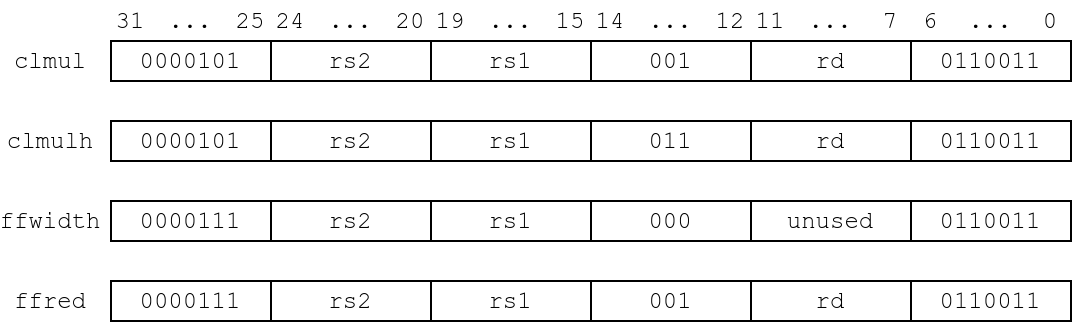
\includegraphics[width=0.8\linewidth]{img/instr.png}
    \caption{The instruction format for the custom Galois field arithmetic instructions.}
    \Description{The instruction format for the custom Galois field arithmetic instructions.}
    \label{fig:instr}
\end{figure*}

\begin{itemize}
    \item \textcolor{blue}{Non-binary error-correction codes (i.e., Non-binary LDPC, BCH, RS codes, \dots)}
    \item \textcolor{blue}{Pre-quantum cryptography (i.e., AES, Elliptic Curve, \dots)}
    \item \textcolor{blue}{PQC cryptography (i.e., McEliece, Rainbow, HQC, \dots)}
\end{itemize}




\section{Proposed ISA extension}

\section{Experiment results}

\section{Conclusions}

%\section{Acknowledgments}

%Identification of funding sources and other support, and thanks to
%individuals and groups that assisted in the research and the
%preparation of the work should be included in an acknowledgment
%section, which is placed just before the reference section in your
%document.

%%
%% The next two lines define the bibliography style to be used, and
%% the bibliography file.
\bibliographystyle{ACM-Reference-Format}
\bibliography{sample-base}



\end{document}
\endinput
%%
%% End of file `sample-sigconf.tex'.
